\documentclass[../../main.tex]{subfiles}
\begin{document}

\begin{flushright}
\footnotesize\textit{【自動文字起こし・要確認】}
\end{flushright}

{\bf [解]}
$\angle A=\theta$とおく．内角の正条件から
\begin{align}
0<\theta，\ 0<2\theta，\ 0<\pi-3\theta \iff 0<\theta<\dfrac{\pi}{3}\quad\cdots①
\end{align}
である．

\begin{figure}[htb]
\centering
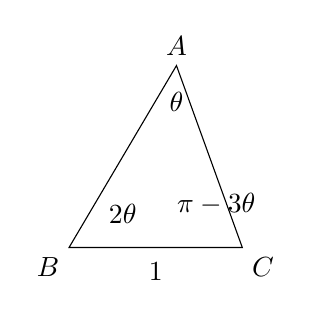
\begin{tikzpicture}[scale=2.2]
  \coordinate (B) at (0,0);
  \coordinate (C) at (1,0);
  \coordinate (A) at (0.62,1.05);
  \draw (A) -- (B) -- (C) -- cycle;
  \node[above] at (A) {$A$};
  \node[below left] at (B) {$B$};
  \node[below right] at (C) {$C$};
  \node[below=2pt] at (0.5,0) {$1$};
  \node[above=2pt] at (0.31,0.05) {$2\theta$};
  \node[above=2pt] at (0.85,0.1) {$\pi-3\theta$};
  \node[below=6pt] at (A) {$\theta$};
\end{tikzpicture}
\caption{$\triangle ABC$と角$\theta$，$2\theta$，$\pi-3\theta$の関係}
\end{figure}

正弦定理より
\begin{align}
\dfrac{\overline{AB}}{\sin(\pi-3\theta)}=\dfrac{1}{\sin\theta}
\quad\therefore\ \overline{AB}=\dfrac{\sin3\theta}{\sin\theta}=3-4\sin^2\theta\quad\cdots②
\end{align}

以下，$c=\cos\theta$，$s=\sin\theta$とする．$\triangle ABC$の面積$T$は②から
\begin{align}
T&=\dfrac{1}{2}\overline{AB}\cdot\overline{BC}\cdot\sin2\theta\\
&=\dfrac{1}{2}(3-4s^2)\cdot2sc\\
&=(3-4s^2)sc
\end{align}

これを$\theta$で微分して，
\begin{align}
T'&=3\cos2\theta-4(3s^2c^2+(-s)\cdot s^3)\\
&=3(1-2s^2)-4s^2(3c^2-s^2)\\
&=3(1-2s^2)-4s^2(3-4s^2)\\
&=16t^2-18t+3\quad(t=s^2)
\end{align}

$16t^2-18t+3=0$を解くと$t=\dfrac{9\pm\sqrt{33}}{16}$であり，①の範囲（$0<t<3/4$）に入るのは$t=\dfrac{9-\sqrt{33}}{16}$のみだから，下表を得る．

\begin{center}
\begin{tabular}{c|ccccc}
$\theta$ & $0$ & & & & $\pi/3$ \\
\hline
$t$ & $0$ & & $\dfrac{9-\sqrt{33}}{16}$ & & $3/4$ \\
\hline
$T'$ & & $+$ & $0$ & $-$ & \\
\hline
$T$ & & $\nearrow$ & （極大） & $\searrow$ & \\
\end{tabular}
\end{center}

したがって，もとめるのは
\begin{align}
\cos\angle B=\cos2\theta=1-2t=1-\dfrac{9-\sqrt{33}}{8}=\dfrac{-1+\sqrt{33}}{8}．
\end{align}

\newpage

\end{document}
